\documentclass[dvipdfmx,cjk]{beamer}
\usepackage{mymacro}
%%\usepackage{emath,emathE,emathEy}
\usepackage[all]{xy}
\usepackage{listings,coqlistings} % Coq
\usepackage{color,tikz,here,mathdots,graphicx} % 図・コード
\usetikzlibrary{intersections,calc,arrows.meta,positioning}

\AtBeginDvi{\special{pdf:tounicode 90ms-RKSJ-UCS2}}
\AtBeginDvi{\special{pdf:tounicode EUC-UCS2}}

\setbeamertemplate{navigation symbols}{} %% 右下のアイコンを消す

%フレーム
%\usetheme{CambridgeUS}
%\usetheme{Boadilla}
\usetheme{Madrid}
%\usetheme{Antibes}
%\usetheme{Montpellier}
%\usetheme{Berkeley}
%\usetheme{Goettingen}
%\usetheme{Singapore}
%\usetheme{Szeged}

%色,フォント,内枠,外枠
%\usecolortheme{rose}
%\usecolortheme{albatross}
%\useoutertheme{shadow}                
\usefonttheme{professionalfonts}

%オプション
%\setbeamercovered{transparent}         %% 消えている文字をうっすらと表示する
\setbeamertemplate{theorems}[numbered] %% theorem 環境の冒頭に番号をつける

% 定理環境
\newtheorem{dfn}{定義}[section]
\newtheorem{thm}[dfn]{定理}
\newtheorem{exm}[dfn]{例}
\newcommand{\redt}[1]{\textcolor{red}{#1}}
\newcommand{\blut}[1]{\textcolor{blue}{#1}}
\renewcommand{\proofname}{証明}

% マクロ
\def\Color{\textit{Color}}
\def\mix{\textit{mix}}
\def\red{\textit{red}}
\def\blu{\textit{blu}}
\def\yel{\textit{yel}}
\def\mix{\textit{mix}}
\def\colorYB{\textit{colorYB}}
\def\colorBYB{\textit{colorBYB}}
\def\colorYBBY{\textit{colorYBBY}}
\def\Cpos{\textit{cpos}}
\def\WCT{\textit{WellColoredTriangle}}
\def\Triangle{\textit{Triangle}}
\def\next{\textit{next}}
\def\mixCut{\textit{mixcut}}
\def\AllRed{\textit{allred}}
\def\falseColor{\textit{falseColor}}
\def\Cexists{\textit{C\_exists}}
\def\Cuniq{\textit{C\_uniq}}
\def\Cmix{\textit{C\_mix}}
\def\Cpaint{\textit{C\_paint}}
\def\EvenA{\textit{EvenA}}
\def\EvenB{\textit{EvenB}}
\def\Even{\textit{Even}}
\def\ShortOddA{\textit{ShortOddA}}
\def\ShortOddB{\textit{ShortOddB}}
\def\ShortOddC{\textit{ShortOddC}}
\def\ShortOdd{\textit{ShortOdd}}
\def\LongOddA{\textit{LongOddA}}
\def\LongOddB{\textit{LongOddB}}
\def\LongOddC{\textit{LongOddC}}
\def\LongOdd{\textit{LongOdd}}


\begin{document}
\title[Coqによる三角形三色問題の証明]{Coqによる三角形三色問題の証明} 
\author[橋本翔太]{橋本 翔太}
\subject{\footnotesize{2021年度情報科学専攻 修士1年中間発表会}}
\institute[木村大輔 研究室]{木村大輔 研究室}
\date[2022年2月17日]{2022年2月17日(木)} %September 1st,2021

% タイトルページ
\begin{frame}
  \titlepage
  \begin{center}
    {\small{2021年度情報科学専攻 修士1年中間発表会}}
  \end{center}
\end{frame}

% 目次
\begin{frame}
  \tableofcontents
\end{frame}

% 本編
\section{研究の背景・概要}

\large
\begin{frame}
  \frametitle{研究の背景}
  Coq \\
  \begin{itemize}
  \item
    人間と対話的に証明を完成させることのできる定理証明支援系
  \end{itemize}
  \vfill
  三角形三色問題
  \begin{itemize}
    \item
    規則に従って塗り分けられた三角形に配置されたマスに
    関する問題
    \item
      『数学セミナー』にて出題(証明済)
      \vfill
    \begin{center}
      \begin{tabular}{ccc}
        % wellcolored
\begin{tikzpicture}[scale=0.25]
  % 左図
  \begin{scope}[xshift={-150}]
    \myHexB{-1}{1}
    \myHexY{1}{1}
    \myHexR{0}{0}
  \end{scope}
  % 右図  
  \begin{scope}[xshift={150}]
    \myHexY{-1}{1}
    \myHexY{1}{1}
    \myHexY{0}{0}
  \end{scope}
\end{tikzpicture}

        &
        \hfill
        &
        \definecolor{grayR}{rgb}{0.10, 0.10, 0.10}
\definecolor{grayB}{rgb}{0.50, 0.50, 0.50}
\definecolor{grayY}{rgb}{1.00, 1.00, 1.00}
%\def\myRed{red}
%\def\myBlue{blue}
%\def\myYellow{yellow}
\def\myRed{grayR}
\def\myBlue{grayB}
\def\myYellow{grayY}

% 9steps

\begin{tikzpicture}[scale=0.25]
  %9段目
  \filldraw[fill=\myRed] (0,0)--++(30:1)--++(90:1)--++(150:1)--++(210:1)--++(270:1)--cycle;
  %8段目
  \filldraw[fill=\myYellow,xshift={-25},yshift={25*sqrt(3)}] (0,0)--++(30:1)--++(90:1)--++(150:1)--++(210:1)--++(270:1)--cycle;
  \filldraw[fill=\myBlue,xshift={25},yshift={25*sqrt(3)}] (0,0)--++(30:1)--++(90:1)--++(150:1)--++(210:1)--++(270:1)--cycle;
  %7段目
  \filldraw[fill=\myYellow,xshift={-25*2},yshift={25*sqrt(3)*2}] (0,0)--++(30:1)--++(90:1)--++(150:1)--++(210:1)--++(270:1)--cycle;
  \filldraw[fill=\myYellow,yshift={25*sqrt(3)*2}] (0,0)--++(30:1)--++(90:1)--++(150:1)--++(210:1)--++(270:1)--cycle;
  \filldraw[fill=\myRed,xshift={25*2},yshift={25*sqrt(3)*2}] (0,0)--++(30:1)--++(90:1)--++(150:1)--++(210:1)--++(270:1)--cycle;
  %6段目
  \filldraw[fill=\myBlue,xshift={-25*3},yshift={25*sqrt(3)*3}] (0,0)--++(30:1)--++(90:1)--++(150:1)--++(210:1)--++(270:1)--cycle;
  \filldraw[fill=\myRed,xshift={-25},yshift={25*sqrt(3)*3}] (0,0)--++(30:1)--++(90:1)--++(150:1)--++(210:1)--++(270:1)--cycle;
  \filldraw[fill=\myBlue,xshift={25},yshift={25*sqrt(3)*3}] (0,0)--++(30:1)--++(90:1)--++(150:1)--++(210:1)--++(270:1)--cycle;
  \filldraw[fill=\myYellow,xshift={25*3},yshift={25*sqrt(3)*3}] (0,0)--++(30:1)--++(90:1)--++(150:1)--++(210:1)--++(270:1)--cycle;
  %5段目
  \filldraw[fill=\myYellow,xshift={-25*4},yshift={25*sqrt(3)*4}] (0,0)--++(30:1)--++(90:1)--++(150:1)--++(210:1)--++(270:1)--cycle;
  \filldraw[fill=\myRed,xshift={-25*2},yshift={25*sqrt(3)*4}] (0,0)--++(30:1)--++(90:1)--++(150:1)--++(210:1)--++(270:1)--cycle;
  \filldraw[fill=\myRed,yshift={25*sqrt(3)*4}] (0,0)--++(30:1)--++(90:1)--++(150:1)--++(210:1)--++(270:1)--cycle;
  \filldraw[fill=\myYellow,xshift={25*2},yshift={25*sqrt(3)*4}] (0,0)--++(30:1)--++(90:1)--++(150:1)--++(210:1)--++(270:1)--cycle;
  \filldraw[fill=\myYellow,xshift={25*4},yshift={25*sqrt(3)*4}] (0,0)--++(30:1)--++(90:1)--++(150:1)--++(210:1)--++(270:1)--cycle;
  %4段目
  \filldraw[fill=\myRed,xshift={-25*5},yshift={25*sqrt(3)*5}] (0,0)--++(30:1)--++(90:1)--++(150:1)--++(210:1)--++(270:1)--cycle;
  \filldraw[fill=\myBlue,xshift={-25*3},yshift={25*sqrt(3)*5}] (0,0)--++(30:1)--++(90:1)--++(150:1)--++(210:1)--++(270:1)--cycle;
  \filldraw[fill=\myYellow,xshift={-25*1},yshift={25*sqrt(3)*5}] (0,0)--++(30:1)--++(90:1)--++(150:1)--++(210:1)--++(270:1)--cycle;
  \filldraw[fill=\myBlue,xshift={25*1},yshift={25*sqrt(3)*5}] (0,0)--++(30:1)--++(90:1)--++(150:1)--++(210:1)--++(270:1)--cycle;
  \filldraw[fill=\myRed,xshift={25*3},yshift={25*sqrt(3)*5}] (0,0)--++(30:1)--++(90:1)--++(150:1)--++(210:1)--++(270:1)--cycle;
  \filldraw[fill=\myBlue,xshift={25*5},yshift={25*sqrt(3)*5}] (0,0)--++(30:1)--++(90:1)--++(150:1)--++(210:1)--++(270:1)--cycle;
  %3段目
  \filldraw[fill=\myRed,xshift={-25*6},yshift={25*sqrt(3)*6}] (0,0)--++(30:1)--++(90:1)--++(150:1)--++(210:1)--++(270:1)--cycle;
  \filldraw[fill=\myRed,xshift={-25*4},yshift={25*sqrt(3)*6}] (0,0)--++(30:1)--++(90:1)--++(150:1)--++(210:1)--++(270:1)--cycle;
  \filldraw[fill=\myYellow,xshift={-25*2},yshift={25*sqrt(3)*6}] (0,0)--++(30:1)--++(90:1)--++(150:1)--++(210:1)--++(270:1)--cycle;
  \filldraw[fill=\myYellow,yshift={25*sqrt(3)*6}] (0,0)--++(30:1)--++(90:1)--++(150:1)--++(210:1)--++(270:1)--cycle;
  \filldraw[fill=\myRed,xshift={25*2},yshift={25*sqrt(3)*6}] (0,0)--++(30:1)--++(90:1)--++(150:1)--++(210:1)--++(270:1)--cycle;
  \filldraw[fill=\myRed,xshift={25*4},yshift={25*sqrt(3)*6}] (0,0)--++(30:1)--++(90:1)--++(150:1)--++(210:1)--++(270:1)--cycle;
  \filldraw[fill=\myYellow,xshift={25*6},yshift={25*sqrt(3)*6}] (0,0)--++(30:1)--++(90:1)--++(150:1)--++(210:1)--++(270:1)--cycle;
  %2段目
  \filldraw[fill=\myBlue,xshift={-25*7},yshift={25*sqrt(3)*7}] (0,0)--++(30:1)--++(90:1)--++(150:1)--++(210:1)--++(270:1)--cycle;
  \filldraw[fill=\myYellow,xshift={-25*5},yshift={25*sqrt(3)*7}] (0,0)--++(30:1)--++(90:1)--++(150:1)--++(210:1)--++(270:1)--cycle;
  \filldraw[fill=\myBlue,xshift={-25*3},yshift={25*sqrt(3)*7}] (0,0)--++(30:1)--++(90:1)--++(150:1)--++(210:1)--++(270:1)--cycle;
  \filldraw[fill=\myRed,xshift={-25*1},yshift={25*sqrt(3)*7}] (0,0)--++(30:1)--++(90:1)--++(150:1)--++(210:1)--++(270:1)--cycle;
  \filldraw[fill=\myBlue,xshift={25*1},yshift={25*sqrt(3)*7}] (0,0)--++(30:1)--++(90:1)--++(150:1)--++(210:1)--++(270:1)--cycle;
  \filldraw[fill=\myYellow,xshift={25*3},yshift={25*sqrt(3)*7}] (0,0)--++(30:1)--++(90:1)--++(150:1)--++(210:1)--++(270:1)--cycle;
  \filldraw[fill=\myBlue,xshift={25*5},yshift={25*sqrt(3)*7}] (0,0)--++(30:1)--++(90:1)--++(150:1)--++(210:1)--++(270:1)--cycle;
  \filldraw[fill=\myRed,xshift={25*7},yshift={25*sqrt(3)*7}] (0,0)--++(30:1)--++(90:1)--++(150:1)--++(210:1)--++(270:1)--cycle;
  %1段目
  \filldraw[fill=\myRed,xshift={-25*8},yshift={25*sqrt(3)*8}] (0,0)--++(30:1)--++(90:1)--++(150:1)--++(210:1)--++(270:1)--cycle;
  \filldraw[fill=\myYellow,xshift={-25*6},yshift={25*sqrt(3)*8}] (0,0)--++(30:1)--++(90:1)--++(150:1)--++(210:1)--++(270:1)--cycle;
  \filldraw[fill=\myYellow,xshift={-25*4},yshift={25*sqrt(3)*8}] (0,0)--++(30:1)--++(90:1)--++(150:1)--++(210:1)--++(270:1)--cycle;
  \filldraw[fill=\myRed,xshift={-25*2},yshift={25*sqrt(3)*8}] (0,0)--++(30:1)--++(90:1)--++(150:1)--++(210:1)--++(270:1)--cycle;
  \filldraw[fill=\myRed,yshift={25*sqrt(3)*8}] (0,0)--++(30:1)--++(90:1)--++(150:1)--++(210:1)--++(270:1)--cycle;
  \filldraw[fill=\myYellow,xshift={25*2},yshift={25*sqrt(3)*8}] (0,0)--++(30:1)--++(90:1)--++(150:1)--++(210:1)--++(270:1)--cycle;
  \filldraw[fill=\myYellow,xshift={25*4},yshift={25*sqrt(3)*8}] (0,0)--++(30:1)--++(90:1)--++(150:1)--++(210:1)--++(270:1)--cycle;
  \filldraw[fill=\myRed,xshift={25*6},yshift={25*sqrt(3)*8}] (0,0)--++(30:1)--++(90:1)--++(150:1)--++(210:1)--++(270:1)--cycle;
  \filldraw[fill=\myRed,xshift={25*8},yshift={25*sqrt(3)*8}] (0,0)--++(30:1)--++(90:1)--++(150:1)--++(210:1)--++(270:1)--cycle;
  %0段目
  \filldraw[fill=\myYellow,xshift={-25*9},yshift={25*sqrt(3)*9}] (0,0)--++(30:1)--++(90:1)--++(150:1)--++(210:1)--++(270:1)--cycle;
  \filldraw[fill=\myBlue,xshift={-25*7},yshift={25*sqrt(3)*9}] (0,0)--++(30:1)--++(90:1)--++(150:1)--++(210:1)--++(270:1)--cycle;
  \filldraw[fill=\myRed,xshift={-25*5},yshift={25*sqrt(3)*9}] (0,0)--++(30:1)--++(90:1)--++(150:1)--++(210:1)--++(270:1)--cycle;
  \filldraw[fill=\myBlue,xshift={-25*3},yshift={25*sqrt(3)*9}] (0,0)--++(30:1)--++(90:1)--++(150:1)--++(210:1)--++(270:1)--cycle;
  \filldraw[fill=\myYellow,xshift={-25*1},yshift={25*sqrt(3)*9}] (0,0)--++(30:1)--++(90:1)--++(150:1)--++(210:1)--++(270:1)--cycle;
  \filldraw[fill=\myBlue,xshift={25*1},yshift={25*sqrt(3)*9}] (0,0)--++(30:1)--++(90:1)--++(150:1)--++(210:1)--++(270:1)--cycle;
  \filldraw[fill=\myRed,xshift={25*3},yshift={25*sqrt(3)*9}] (0,0)--++(30:1)--++(90:1)--++(150:1)--++(210:1)--++(270:1)--cycle;
  \filldraw[fill=\myBlue,xshift={25*5},yshift={25*sqrt(3)*9}] (0,0)--++(30:1)--++(90:1)--++(150:1)--++(210:1)--++(270:1)--cycle;
  \filldraw[fill=\myYellow,xshift={25*7},yshift={25*sqrt(3)*9}] (0,0)--++(30:1)--++(90:1)--++(150:1)--++(210:1)--++(270:1)--cycle;
  \filldraw[fill=\myBlue,xshift={25*9},yshift={25*sqrt(3)*9}] (0,0)--++(30:1)--++(90:1)--++(150:1)--++(210:1)--++(270:1)--cycle;
\end{tikzpicture}

        \\
        色塗り規則
        &
        \hfill
        &
        色の塗られた三角形
      \end{tabular}
    \end{center}
  \end{itemize}
\end{frame}

\begin{frame}
  \frametitle{研究の背景}
  \begin{block}{Coq}
    人間と対話的に証明を完成させることのできる定理証明支援系
  \end{block}
  \vfill
  \begin{minipage}{0.45\hsize}
    \begin{center}
      \begin{exampleblock}{ Coq の利点}
        \begin{itemize}
        \item 証明の受け渡しが容易
        \item 機械的操作のミスを排除
        \item 場合分けの漏れの防止
        \item 簡単な主張は自動証明
        \end{itemize}
      \end{exampleblock}
    \end{center}
    \vfill
  \end{minipage}
  \hfill
  \begin{minipage}{0.45\hsize}
    \begin{center}
      \includegraphics[width=5.5cm]{coq_example.png} \\
      Coqの表示画面
      \vfill
    \end{center}
  \end{minipage}
  \hfill
\end{frame}

\begin{frame}
  \frametitle{研究の背景}
  \begin{block}{調和性}
    $3$つのマスに塗られている色がすべて同じか相異なるとき,
    この$3$マスは調和しているという.
  \end{block}
  \[
  \begin{tabular}{ccc}
      % wellcolored
\begin{tikzpicture}[scale=0.25]
  % 左図
  \begin{scope}[xshift={-150}]
    \myHexB{-1}{1}
    \myHexY{1}{1}
    \myHexR{0}{0}
  \end{scope}
  % 右図  
  \begin{scope}[xshift={150}]
    \myHexY{-1}{1}
    \myHexY{1}{1}
    \myHexY{0}{0}
  \end{scope}
\end{tikzpicture}

      &
      \hfill
      &
      \definecolor{grayR}{rgb}{0.50, 0.50, 0.50}
\definecolor{grayB}{rgb}{0.10, 0.10, 0.10}
\definecolor{grayY}{rgb}{1.00, 1.00, 1.00}
%\def\myRed{red}
%\def\myBlue{blue}
%\def\myYellow{yellow}
\def\myRed{grayR}
\def\myBlue{grayB}
\def\myYellow{grayY}

% wellcolored

\begin{tikzpicture}[scale=0.25]
  %1段目
  \filldraw[fill=\myRed,xshift={-25*5},yshift={25*sqrt(3)*3}] (0,0)--++(30:1)--++(90:1)--++(150:1)--++(210:1)--++(270:1)--cycle;
  \filldraw[fill=\myYellow,xshift={25*5},yshift={25*sqrt(3)*3}] (0,0)--++(30:1)--++(90:1)--++(150:1)--++(210:1)--++(270:1)--cycle;
  %0段目
  \filldraw[fill=\myBlue,xshift={-25*4},yshift={25*sqrt(3)*4}] (0,0)--++(30:1)--++(90:1)--++(150:1)--++(210:1)--++(270:1)--cycle;
  \filldraw[fill=\myBlue,xshift={-25*6},yshift={25*sqrt(3)*4}] (0,0)--++(30:1)--++(90:1)--++(150:1)--++(210:1)--++(270:1)--cycle;
  \filldraw[fill=\myYellow,xshift={25*6},yshift={25*sqrt(3)*4}] (0,0)--++(30:1)--++(90:1)--++(150:1)--++(210:1)--++(270:1)--cycle;
  \filldraw[fill=\myRed,xshift={25*4},yshift={25*sqrt(3)*4}] (0,0)--++(30:1)--++(90:1)--++(150:1)--++(210:1)--++(270:1)--cycle;
\end{tikzpicture}

      \\
      調和性を満たす
      &
      \hfill
      &
      調和性を満たさない
  \end{tabular}
  \]
  \begin{block}{調和彩色三角形}
    $3$つの端点のマスに塗られている色が調和性を満たしている三色三角形を
    調和彩色三角形 (Well-Colored Triangle) という.
  \end{block}
  \vfill
\end{frame}

\normalsize
\begin{frame}
  \frametitle{研究の背景}
  \begin{block}{三角形三色問題(数学セミナー)}
    最上段のマスのどのような塗り方に対しても
    調和彩色三角形になる段数 $n$ を求めよ.
    \\
    \textbf{[解答]}$n=3^k$のとき(証明済)
  \end{block}
  \[
  \begin{tabular}{ccc}
    \input{four_steps}
    &
    \definecolor{grayR}{rgb}{0.10, 0.10, 0.10}
\definecolor{grayB}{rgb}{0.50, 0.50, 0.50}
\definecolor{grayY}{rgb}{1.00, 1.00, 1.00}
%\def\myRed{red}
%\def\myBlue{blue}
%\def\myYellow{yellow}
\def\myRed{grayR}
\def\myBlue{grayB}
\def\myYellow{grayY}

% 9steps

\begin{tikzpicture}[scale=0.25]
  %9段目
  \filldraw[fill=\myRed] (0,0)--++(30:1)--++(90:1)--++(150:1)--++(210:1)--++(270:1)--cycle;
  %8段目
  \filldraw[fill=\myYellow,xshift={-25},yshift={25*sqrt(3)}] (0,0)--++(30:1)--++(90:1)--++(150:1)--++(210:1)--++(270:1)--cycle;
  \filldraw[fill=\myBlue,xshift={25},yshift={25*sqrt(3)}] (0,0)--++(30:1)--++(90:1)--++(150:1)--++(210:1)--++(270:1)--cycle;
  %7段目
  \filldraw[fill=\myYellow,xshift={-25*2},yshift={25*sqrt(3)*2}] (0,0)--++(30:1)--++(90:1)--++(150:1)--++(210:1)--++(270:1)--cycle;
  \filldraw[fill=\myYellow,yshift={25*sqrt(3)*2}] (0,0)--++(30:1)--++(90:1)--++(150:1)--++(210:1)--++(270:1)--cycle;
  \filldraw[fill=\myRed,xshift={25*2},yshift={25*sqrt(3)*2}] (0,0)--++(30:1)--++(90:1)--++(150:1)--++(210:1)--++(270:1)--cycle;
  %6段目
  \filldraw[fill=\myBlue,xshift={-25*3},yshift={25*sqrt(3)*3}] (0,0)--++(30:1)--++(90:1)--++(150:1)--++(210:1)--++(270:1)--cycle;
  \filldraw[fill=\myRed,xshift={-25},yshift={25*sqrt(3)*3}] (0,0)--++(30:1)--++(90:1)--++(150:1)--++(210:1)--++(270:1)--cycle;
  \filldraw[fill=\myBlue,xshift={25},yshift={25*sqrt(3)*3}] (0,0)--++(30:1)--++(90:1)--++(150:1)--++(210:1)--++(270:1)--cycle;
  \filldraw[fill=\myYellow,xshift={25*3},yshift={25*sqrt(3)*3}] (0,0)--++(30:1)--++(90:1)--++(150:1)--++(210:1)--++(270:1)--cycle;
  %5段目
  \filldraw[fill=\myYellow,xshift={-25*4},yshift={25*sqrt(3)*4}] (0,0)--++(30:1)--++(90:1)--++(150:1)--++(210:1)--++(270:1)--cycle;
  \filldraw[fill=\myRed,xshift={-25*2},yshift={25*sqrt(3)*4}] (0,0)--++(30:1)--++(90:1)--++(150:1)--++(210:1)--++(270:1)--cycle;
  \filldraw[fill=\myRed,yshift={25*sqrt(3)*4}] (0,0)--++(30:1)--++(90:1)--++(150:1)--++(210:1)--++(270:1)--cycle;
  \filldraw[fill=\myYellow,xshift={25*2},yshift={25*sqrt(3)*4}] (0,0)--++(30:1)--++(90:1)--++(150:1)--++(210:1)--++(270:1)--cycle;
  \filldraw[fill=\myYellow,xshift={25*4},yshift={25*sqrt(3)*4}] (0,0)--++(30:1)--++(90:1)--++(150:1)--++(210:1)--++(270:1)--cycle;
  %4段目
  \filldraw[fill=\myRed,xshift={-25*5},yshift={25*sqrt(3)*5}] (0,0)--++(30:1)--++(90:1)--++(150:1)--++(210:1)--++(270:1)--cycle;
  \filldraw[fill=\myBlue,xshift={-25*3},yshift={25*sqrt(3)*5}] (0,0)--++(30:1)--++(90:1)--++(150:1)--++(210:1)--++(270:1)--cycle;
  \filldraw[fill=\myYellow,xshift={-25*1},yshift={25*sqrt(3)*5}] (0,0)--++(30:1)--++(90:1)--++(150:1)--++(210:1)--++(270:1)--cycle;
  \filldraw[fill=\myBlue,xshift={25*1},yshift={25*sqrt(3)*5}] (0,0)--++(30:1)--++(90:1)--++(150:1)--++(210:1)--++(270:1)--cycle;
  \filldraw[fill=\myRed,xshift={25*3},yshift={25*sqrt(3)*5}] (0,0)--++(30:1)--++(90:1)--++(150:1)--++(210:1)--++(270:1)--cycle;
  \filldraw[fill=\myBlue,xshift={25*5},yshift={25*sqrt(3)*5}] (0,0)--++(30:1)--++(90:1)--++(150:1)--++(210:1)--++(270:1)--cycle;
  %3段目
  \filldraw[fill=\myRed,xshift={-25*6},yshift={25*sqrt(3)*6}] (0,0)--++(30:1)--++(90:1)--++(150:1)--++(210:1)--++(270:1)--cycle;
  \filldraw[fill=\myRed,xshift={-25*4},yshift={25*sqrt(3)*6}] (0,0)--++(30:1)--++(90:1)--++(150:1)--++(210:1)--++(270:1)--cycle;
  \filldraw[fill=\myYellow,xshift={-25*2},yshift={25*sqrt(3)*6}] (0,0)--++(30:1)--++(90:1)--++(150:1)--++(210:1)--++(270:1)--cycle;
  \filldraw[fill=\myYellow,yshift={25*sqrt(3)*6}] (0,0)--++(30:1)--++(90:1)--++(150:1)--++(210:1)--++(270:1)--cycle;
  \filldraw[fill=\myRed,xshift={25*2},yshift={25*sqrt(3)*6}] (0,0)--++(30:1)--++(90:1)--++(150:1)--++(210:1)--++(270:1)--cycle;
  \filldraw[fill=\myRed,xshift={25*4},yshift={25*sqrt(3)*6}] (0,0)--++(30:1)--++(90:1)--++(150:1)--++(210:1)--++(270:1)--cycle;
  \filldraw[fill=\myYellow,xshift={25*6},yshift={25*sqrt(3)*6}] (0,0)--++(30:1)--++(90:1)--++(150:1)--++(210:1)--++(270:1)--cycle;
  %2段目
  \filldraw[fill=\myBlue,xshift={-25*7},yshift={25*sqrt(3)*7}] (0,0)--++(30:1)--++(90:1)--++(150:1)--++(210:1)--++(270:1)--cycle;
  \filldraw[fill=\myYellow,xshift={-25*5},yshift={25*sqrt(3)*7}] (0,0)--++(30:1)--++(90:1)--++(150:1)--++(210:1)--++(270:1)--cycle;
  \filldraw[fill=\myBlue,xshift={-25*3},yshift={25*sqrt(3)*7}] (0,0)--++(30:1)--++(90:1)--++(150:1)--++(210:1)--++(270:1)--cycle;
  \filldraw[fill=\myRed,xshift={-25*1},yshift={25*sqrt(3)*7}] (0,0)--++(30:1)--++(90:1)--++(150:1)--++(210:1)--++(270:1)--cycle;
  \filldraw[fill=\myBlue,xshift={25*1},yshift={25*sqrt(3)*7}] (0,0)--++(30:1)--++(90:1)--++(150:1)--++(210:1)--++(270:1)--cycle;
  \filldraw[fill=\myYellow,xshift={25*3},yshift={25*sqrt(3)*7}] (0,0)--++(30:1)--++(90:1)--++(150:1)--++(210:1)--++(270:1)--cycle;
  \filldraw[fill=\myBlue,xshift={25*5},yshift={25*sqrt(3)*7}] (0,0)--++(30:1)--++(90:1)--++(150:1)--++(210:1)--++(270:1)--cycle;
  \filldraw[fill=\myRed,xshift={25*7},yshift={25*sqrt(3)*7}] (0,0)--++(30:1)--++(90:1)--++(150:1)--++(210:1)--++(270:1)--cycle;
  %1段目
  \filldraw[fill=\myRed,xshift={-25*8},yshift={25*sqrt(3)*8}] (0,0)--++(30:1)--++(90:1)--++(150:1)--++(210:1)--++(270:1)--cycle;
  \filldraw[fill=\myYellow,xshift={-25*6},yshift={25*sqrt(3)*8}] (0,0)--++(30:1)--++(90:1)--++(150:1)--++(210:1)--++(270:1)--cycle;
  \filldraw[fill=\myYellow,xshift={-25*4},yshift={25*sqrt(3)*8}] (0,0)--++(30:1)--++(90:1)--++(150:1)--++(210:1)--++(270:1)--cycle;
  \filldraw[fill=\myRed,xshift={-25*2},yshift={25*sqrt(3)*8}] (0,0)--++(30:1)--++(90:1)--++(150:1)--++(210:1)--++(270:1)--cycle;
  \filldraw[fill=\myRed,yshift={25*sqrt(3)*8}] (0,0)--++(30:1)--++(90:1)--++(150:1)--++(210:1)--++(270:1)--cycle;
  \filldraw[fill=\myYellow,xshift={25*2},yshift={25*sqrt(3)*8}] (0,0)--++(30:1)--++(90:1)--++(150:1)--++(210:1)--++(270:1)--cycle;
  \filldraw[fill=\myYellow,xshift={25*4},yshift={25*sqrt(3)*8}] (0,0)--++(30:1)--++(90:1)--++(150:1)--++(210:1)--++(270:1)--cycle;
  \filldraw[fill=\myRed,xshift={25*6},yshift={25*sqrt(3)*8}] (0,0)--++(30:1)--++(90:1)--++(150:1)--++(210:1)--++(270:1)--cycle;
  \filldraw[fill=\myRed,xshift={25*8},yshift={25*sqrt(3)*8}] (0,0)--++(30:1)--++(90:1)--++(150:1)--++(210:1)--++(270:1)--cycle;
  %0段目
  \filldraw[fill=\myYellow,xshift={-25*9},yshift={25*sqrt(3)*9}] (0,0)--++(30:1)--++(90:1)--++(150:1)--++(210:1)--++(270:1)--cycle;
  \filldraw[fill=\myBlue,xshift={-25*7},yshift={25*sqrt(3)*9}] (0,0)--++(30:1)--++(90:1)--++(150:1)--++(210:1)--++(270:1)--cycle;
  \filldraw[fill=\myRed,xshift={-25*5},yshift={25*sqrt(3)*9}] (0,0)--++(30:1)--++(90:1)--++(150:1)--++(210:1)--++(270:1)--cycle;
  \filldraw[fill=\myBlue,xshift={-25*3},yshift={25*sqrt(3)*9}] (0,0)--++(30:1)--++(90:1)--++(150:1)--++(210:1)--++(270:1)--cycle;
  \filldraw[fill=\myYellow,xshift={-25*1},yshift={25*sqrt(3)*9}] (0,0)--++(30:1)--++(90:1)--++(150:1)--++(210:1)--++(270:1)--cycle;
  \filldraw[fill=\myBlue,xshift={25*1},yshift={25*sqrt(3)*9}] (0,0)--++(30:1)--++(90:1)--++(150:1)--++(210:1)--++(270:1)--cycle;
  \filldraw[fill=\myRed,xshift={25*3},yshift={25*sqrt(3)*9}] (0,0)--++(30:1)--++(90:1)--++(150:1)--++(210:1)--++(270:1)--cycle;
  \filldraw[fill=\myBlue,xshift={25*5},yshift={25*sqrt(3)*9}] (0,0)--++(30:1)--++(90:1)--++(150:1)--++(210:1)--++(270:1)--cycle;
  \filldraw[fill=\myYellow,xshift={25*7},yshift={25*sqrt(3)*9}] (0,0)--++(30:1)--++(90:1)--++(150:1)--++(210:1)--++(270:1)--cycle;
  \filldraw[fill=\myBlue,xshift={25*9},yshift={25*sqrt(3)*9}] (0,0)--++(30:1)--++(90:1)--++(150:1)--++(210:1)--++(270:1)--cycle;
\end{tikzpicture}

    \\
    段数$n=4$
    &
    段数$n=9$
    \\
    調和彩色三角形でない
    &
    調和彩色三角形である
  \end{tabular}
  \]
  \vfill
\end{frame}

\begin{frame}[fragile]
  \frametitle{研究の概要}
  \begin{block}{研究の成果}
    %% $\forall n, x \in \N, n > 0 \Rightarrow$
    %% $((\exists k \in \N, n = 3 ^ k) \Leftrightarrow \WCT(n,x))$
    {\tt{n > 0 $\Rightarrow$ ($\exists$k, n = 3\verb|^|k) $\Leftrightarrow$ WellColoredTriangle x n}}
    を Coq で証明した.
  \end{block}
  \vfill
  \begin{alertblock}{問題であった点}
    \begin{itemize}
    \item
      幾何的な問題をどのようにして形式化するか
    \item
      暗黙のうちに仮定されてしまっていることを見落としやすい
    \end{itemize}
  \end{alertblock}
  \vfill
  \textbf{[解決法・工夫点]}
  \begin{itemize}
  \item
    三角形三色問題の暗黙の前提を明確化
  \item
    幾何的な状況を関数を用いて論理式で表現
  \end{itemize}
\end{frame}

\section{定義}

\begin{frame}[fragile]
  \frametitle{定義}
  \begin{block}{集合{\tt{Color}}}
    マスに塗る色の集合{\tt{Color}}の定義を以下で与える:
    \begin{lstlisting}[language=Coq]
      Inductive Color : Set := red | yel | blu.
    \end{lstlisting}
  \end{block}
  \begin{block}{彩色関数{\tt{colfun}}}
    {\tt{nat -> nat -> Color}}を型にもつ関数
  \end{block}
  {\tt{colfun x y}}は左から{\tt{x}}番目,上から{\tt{y}}段目のマスに塗る色を表す.
  \vfill  
  \begin{minipage}{0.45\hsize}
  \[
  \definecolor{grayR}{rgb}{0.10, 0.10, 0.10}
\definecolor{grayB}{rgb}{0.50, 0.50, 0.50}
\definecolor{grayY}{rgb}{1.00, 1.00, 1.00}
%\def\myRed{red}
%\def\myBlue{blue}
%\def\myYellow{yellow}
\def\myRed{grayR}
\def\myBlue{grayB}
\def\myYellow{grayY}

% 9steps

\begin{tikzpicture}[scale=0.25]
  %9段目
  \filldraw[fill=\myRed] (0,0)--++(30:1)--++(90:1)--++(150:1)--++(210:1)--++(270:1)--cycle;
  %8段目
  \filldraw[fill=\myYellow,xshift={-25},yshift={25*sqrt(3)}] (0,0)--++(30:1)--++(90:1)--++(150:1)--++(210:1)--++(270:1)--cycle;
  \filldraw[fill=\myBlue,xshift={25},yshift={25*sqrt(3)}] (0,0)--++(30:1)--++(90:1)--++(150:1)--++(210:1)--++(270:1)--cycle;
  %7段目
  \filldraw[fill=\myYellow,xshift={-25*2},yshift={25*sqrt(3)*2}] (0,0)--++(30:1)--++(90:1)--++(150:1)--++(210:1)--++(270:1)--cycle;
  \filldraw[fill=\myYellow,yshift={25*sqrt(3)*2}] (0,0)--++(30:1)--++(90:1)--++(150:1)--++(210:1)--++(270:1)--cycle;
  \filldraw[fill=\myRed,xshift={25*2},yshift={25*sqrt(3)*2}] (0,0)--++(30:1)--++(90:1)--++(150:1)--++(210:1)--++(270:1)--cycle;
  %6段目
  \filldraw[fill=\myBlue,xshift={-25*3},yshift={25*sqrt(3)*3}] (0,0)--++(30:1)--++(90:1)--++(150:1)--++(210:1)--++(270:1)--cycle;
  \filldraw[fill=\myRed,xshift={-25},yshift={25*sqrt(3)*3}] (0,0)--++(30:1)--++(90:1)--++(150:1)--++(210:1)--++(270:1)--cycle;
  \filldraw[fill=\myBlue,xshift={25},yshift={25*sqrt(3)*3}] (0,0)--++(30:1)--++(90:1)--++(150:1)--++(210:1)--++(270:1)--cycle;
  \filldraw[fill=\myYellow,xshift={25*3},yshift={25*sqrt(3)*3}] (0,0)--++(30:1)--++(90:1)--++(150:1)--++(210:1)--++(270:1)--cycle;
  %5段目
  \filldraw[fill=\myYellow,xshift={-25*4},yshift={25*sqrt(3)*4}] (0,0)--++(30:1)--++(90:1)--++(150:1)--++(210:1)--++(270:1)--cycle;
  \filldraw[fill=\myRed,xshift={-25*2},yshift={25*sqrt(3)*4}] (0,0)--++(30:1)--++(90:1)--++(150:1)--++(210:1)--++(270:1)--cycle;
  \filldraw[fill=\myRed,yshift={25*sqrt(3)*4}] (0,0)--++(30:1)--++(90:1)--++(150:1)--++(210:1)--++(270:1)--cycle;
  \filldraw[fill=\myYellow,xshift={25*2},yshift={25*sqrt(3)*4}] (0,0)--++(30:1)--++(90:1)--++(150:1)--++(210:1)--++(270:1)--cycle;
  \filldraw[fill=\myYellow,xshift={25*4},yshift={25*sqrt(3)*4}] (0,0)--++(30:1)--++(90:1)--++(150:1)--++(210:1)--++(270:1)--cycle;
  %4段目
  \filldraw[fill=\myRed,xshift={-25*5},yshift={25*sqrt(3)*5}] (0,0)--++(30:1)--++(90:1)--++(150:1)--++(210:1)--++(270:1)--cycle;
  \filldraw[fill=\myBlue,xshift={-25*3},yshift={25*sqrt(3)*5}] (0,0)--++(30:1)--++(90:1)--++(150:1)--++(210:1)--++(270:1)--cycle;
  \filldraw[fill=\myYellow,xshift={-25*1},yshift={25*sqrt(3)*5}] (0,0)--++(30:1)--++(90:1)--++(150:1)--++(210:1)--++(270:1)--cycle;
  \filldraw[fill=\myBlue,xshift={25*1},yshift={25*sqrt(3)*5}] (0,0)--++(30:1)--++(90:1)--++(150:1)--++(210:1)--++(270:1)--cycle;
  \filldraw[fill=\myRed,xshift={25*3},yshift={25*sqrt(3)*5}] (0,0)--++(30:1)--++(90:1)--++(150:1)--++(210:1)--++(270:1)--cycle;
  \filldraw[fill=\myBlue,xshift={25*5},yshift={25*sqrt(3)*5}] (0,0)--++(30:1)--++(90:1)--++(150:1)--++(210:1)--++(270:1)--cycle;
  %3段目
  \filldraw[fill=\myRed,xshift={-25*6},yshift={25*sqrt(3)*6}] (0,0)--++(30:1)--++(90:1)--++(150:1)--++(210:1)--++(270:1)--cycle;
  \filldraw[fill=\myRed,xshift={-25*4},yshift={25*sqrt(3)*6}] (0,0)--++(30:1)--++(90:1)--++(150:1)--++(210:1)--++(270:1)--cycle;
  \filldraw[fill=\myYellow,xshift={-25*2},yshift={25*sqrt(3)*6}] (0,0)--++(30:1)--++(90:1)--++(150:1)--++(210:1)--++(270:1)--cycle;
  \filldraw[fill=\myYellow,yshift={25*sqrt(3)*6}] (0,0)--++(30:1)--++(90:1)--++(150:1)--++(210:1)--++(270:1)--cycle;
  \filldraw[fill=\myRed,xshift={25*2},yshift={25*sqrt(3)*6}] (0,0)--++(30:1)--++(90:1)--++(150:1)--++(210:1)--++(270:1)--cycle;
  \filldraw[fill=\myRed,xshift={25*4},yshift={25*sqrt(3)*6}] (0,0)--++(30:1)--++(90:1)--++(150:1)--++(210:1)--++(270:1)--cycle;
  \filldraw[fill=\myYellow,xshift={25*6},yshift={25*sqrt(3)*6}] (0,0)--++(30:1)--++(90:1)--++(150:1)--++(210:1)--++(270:1)--cycle;
  %2段目
  \filldraw[fill=\myBlue,xshift={-25*7},yshift={25*sqrt(3)*7}] (0,0)--++(30:1)--++(90:1)--++(150:1)--++(210:1)--++(270:1)--cycle;
  \filldraw[fill=\myYellow,xshift={-25*5},yshift={25*sqrt(3)*7}] (0,0)--++(30:1)--++(90:1)--++(150:1)--++(210:1)--++(270:1)--cycle;
  \filldraw[fill=\myBlue,xshift={-25*3},yshift={25*sqrt(3)*7}] (0,0)--++(30:1)--++(90:1)--++(150:1)--++(210:1)--++(270:1)--cycle;
  \filldraw[fill=\myRed,xshift={-25*1},yshift={25*sqrt(3)*7}] (0,0)--++(30:1)--++(90:1)--++(150:1)--++(210:1)--++(270:1)--cycle;
  \filldraw[fill=\myBlue,xshift={25*1},yshift={25*sqrt(3)*7}] (0,0)--++(30:1)--++(90:1)--++(150:1)--++(210:1)--++(270:1)--cycle;
  \filldraw[fill=\myYellow,xshift={25*3},yshift={25*sqrt(3)*7}] (0,0)--++(30:1)--++(90:1)--++(150:1)--++(210:1)--++(270:1)--cycle;
  \filldraw[fill=\myBlue,xshift={25*5},yshift={25*sqrt(3)*7}] (0,0)--++(30:1)--++(90:1)--++(150:1)--++(210:1)--++(270:1)--cycle;
  \filldraw[fill=\myRed,xshift={25*7},yshift={25*sqrt(3)*7}] (0,0)--++(30:1)--++(90:1)--++(150:1)--++(210:1)--++(270:1)--cycle;
  %1段目
  \filldraw[fill=\myRed,xshift={-25*8},yshift={25*sqrt(3)*8}] (0,0)--++(30:1)--++(90:1)--++(150:1)--++(210:1)--++(270:1)--cycle;
  \filldraw[fill=\myYellow,xshift={-25*6},yshift={25*sqrt(3)*8}] (0,0)--++(30:1)--++(90:1)--++(150:1)--++(210:1)--++(270:1)--cycle;
  \filldraw[fill=\myYellow,xshift={-25*4},yshift={25*sqrt(3)*8}] (0,0)--++(30:1)--++(90:1)--++(150:1)--++(210:1)--++(270:1)--cycle;
  \filldraw[fill=\myRed,xshift={-25*2},yshift={25*sqrt(3)*8}] (0,0)--++(30:1)--++(90:1)--++(150:1)--++(210:1)--++(270:1)--cycle;
  \filldraw[fill=\myRed,yshift={25*sqrt(3)*8}] (0,0)--++(30:1)--++(90:1)--++(150:1)--++(210:1)--++(270:1)--cycle;
  \filldraw[fill=\myYellow,xshift={25*2},yshift={25*sqrt(3)*8}] (0,0)--++(30:1)--++(90:1)--++(150:1)--++(210:1)--++(270:1)--cycle;
  \filldraw[fill=\myYellow,xshift={25*4},yshift={25*sqrt(3)*8}] (0,0)--++(30:1)--++(90:1)--++(150:1)--++(210:1)--++(270:1)--cycle;
  \filldraw[fill=\myRed,xshift={25*6},yshift={25*sqrt(3)*8}] (0,0)--++(30:1)--++(90:1)--++(150:1)--++(210:1)--++(270:1)--cycle;
  \filldraw[fill=\myRed,xshift={25*8},yshift={25*sqrt(3)*8}] (0,0)--++(30:1)--++(90:1)--++(150:1)--++(210:1)--++(270:1)--cycle;
  %0段目
  \filldraw[fill=\myYellow,xshift={-25*9},yshift={25*sqrt(3)*9}] (0,0)--++(30:1)--++(90:1)--++(150:1)--++(210:1)--++(270:1)--cycle;
  \filldraw[fill=\myBlue,xshift={-25*7},yshift={25*sqrt(3)*9}] (0,0)--++(30:1)--++(90:1)--++(150:1)--++(210:1)--++(270:1)--cycle;
  \filldraw[fill=\myRed,xshift={-25*5},yshift={25*sqrt(3)*9}] (0,0)--++(30:1)--++(90:1)--++(150:1)--++(210:1)--++(270:1)--cycle;
  \filldraw[fill=\myBlue,xshift={-25*3},yshift={25*sqrt(3)*9}] (0,0)--++(30:1)--++(90:1)--++(150:1)--++(210:1)--++(270:1)--cycle;
  \filldraw[fill=\myYellow,xshift={-25*1},yshift={25*sqrt(3)*9}] (0,0)--++(30:1)--++(90:1)--++(150:1)--++(210:1)--++(270:1)--cycle;
  \filldraw[fill=\myBlue,xshift={25*1},yshift={25*sqrt(3)*9}] (0,0)--++(30:1)--++(90:1)--++(150:1)--++(210:1)--++(270:1)--cycle;
  \filldraw[fill=\myRed,xshift={25*3},yshift={25*sqrt(3)*9}] (0,0)--++(30:1)--++(90:1)--++(150:1)--++(210:1)--++(270:1)--cycle;
  \filldraw[fill=\myBlue,xshift={25*5},yshift={25*sqrt(3)*9}] (0,0)--++(30:1)--++(90:1)--++(150:1)--++(210:1)--++(270:1)--cycle;
  \filldraw[fill=\myYellow,xshift={25*7},yshift={25*sqrt(3)*9}] (0,0)--++(30:1)--++(90:1)--++(150:1)--++(210:1)--++(270:1)--cycle;
  \filldraw[fill=\myBlue,xshift={25*9},yshift={25*sqrt(3)*9}] (0,0)--++(30:1)--++(90:1)--++(150:1)--++(210:1)--++(270:1)--cycle;
\end{tikzpicture}

  \]
  \end{minipage}
  \begin{minipage}{0.45\hsize}
    左の調和彩色三角形において,
    \begin{itemize}
    \item
      {\tt{colfun 0 0 = yel}}
    \item
      {\tt{colfun 9 0 = blu}}
    \item
      {\tt{colfun 0 9 = red}}
    \end{itemize}
    \hfill
  \end{minipage}
\end{frame}

\begin{frame}[fragile]
  \frametitle{定義とその性質}
  \begin{block}{関数{\tt{mix}}}
    関数{\tt{mix}}の定義を以下で与える:
     \begin{lstlisting}[language=Coq]
      Definition mix c0 c1 :=
      match c0, c1 with
      | red, red => red
      | red, yel => blu
      | red, blu => yel
      | yel, red => blu
      | yel, yel => yel
      | yel, blu => red
      | blu, red => yel
      | blu, yel => red
      | blu, blu => blu
      end.
    \end{lstlisting}
    %% \begin{center}
    %% \begin{tabular}{ccccc}
    %%   $(\red,\red) \Pto \red,$ & $(\red,\yel) \Pto \blu,$ & $(\red,\blu) \Pto \yel,$ \\
    %%   $(\yel,\red) \Pto \blu,$ & $(\yel,\yel) \Pto \yel,$ & $(\yel,\blu) \Pto \red,$ \\
    %%   $(\blu,\red) \Pto \yel,$ & $(\blu,\yel) \Pto \red,$ & $(\blu,\blu) \Pto \blu.$ \\
    %% \end{tabular}
    %% \end{center}
  \end{block}
  %% \begin{exampleblock}{補題$\mixCut$($\mix$の性質)}
  %%   $\forall c_0, c_1, c_2, c_3 \in Color,$ \\
  %%   $\mix( \mix ( \mix(c_0,c_1) , \mix(c_1,c_2) ), \mix( \mix(c_1 c_2),$
  %%   $\mix(c_2,c_3) ) )$ $=$ $\mix(c_0,c_3)$.
  %% \end{exampleblock}
  %% \[
  %% \xymatrix@R=5pt@C=10pt{
  %%   \text{(左辺)} \ar@{-}[r] \ar@{-}[rdd]
  %%   &
  %%   \mix ( \mix(c_0,c_1) , \mix(c_1,c_2) ) \ar@{-}[r] \ar@{-}[rd]
  %%   &
  %%   \mix(c_0,c_1) \ar@{-}[r] \ar@{-}[rd]
  %%   &
  %%   c_0
  %%   \\
  %%   &
  %%   &
  %%   \mix(c_1,c_2) \ar@{-}[r] \ar@{-}[rd]
  %%   &
  %%   c_1
  %%   \\
  %%   &
  %%   \mix( \mix(c_1,c_2), \mix(c_2,c_3) ) ) \ar@{-}[r] \ar@{-}[rd]
  %%   &
  %%   \mix(c_1,c_2) \ar@{-}[r] \ar@{-}[ru]
  %%   &
  %%   c_2
  %%   \\
  %%   &
  %%   &
  %%   \mix(c_2,c_3) \ar@{-}[r] \ar@{-}[ru]
  %%   &
  %%   c_3
  %% }
  %% \]
  %% }
\end{frame}

\begin{frame}[fragile]
  \frametitle{定義}
  \begin{block}{述語{\tt{CFun}},{\tt{Triangle}},{\tt{WellColoredTriangle}}}
    述語{\tt{CFun}},{\tt{Triangle}},{\tt{WellColoredTriangle}}の定義を以下で与える:
  \begin{lstlisting}[language=Coq]
    Definition CFun colfun :=
      forall x y, colfun x y.+1 = mix (colfun x y) (colfun x.+1 y)
    Definition Triangle colfun x y n :=
      colfun x (y + n) = mix (colfun x y) (colfun (x + n) y)
    Definition WellColoredTriangle x n :=
      forall colfun, CFun colfun -> Triangle colfun x 0 n
  \end{lstlisting}
  \end{block}
  \vfill
  \begin{minipage}{0.7\hsize}
    上記の述語は以下を表している:
    \begin{itemize}
    \item
      \small
      {\tt{CFun}}$\cdots$互いに隣接する3マスは調和性を満たす.
    \item
      \small
      {\tt{Triangle}}$\cdots$3つの端点のマスが調和性を満たす.
    \item
      \small
      {\tt{WellColoredTriangle}}$\cdots$調和彩色三角形である.
    \end{itemize}
  \end{minipage}
  \begin{minipage}{0.25\hsize}
    \[
    % 9steps
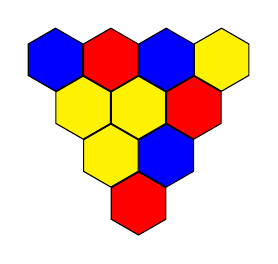
\begin{tikzpicture}[scale=0.4]
  %9段目
  \filldraw[fill=red] (0,0)--++(30:1)--++(90:1)--++(150:1)--++(210:1)--++(270:1)--cycle;
  %8段目
  \filldraw[fill=yellow,xshift={-25},yshift={25*sqrt(3)}] (0,0)--++(30:1)--++(90:1)--++(150:1)--++(210:1)--++(270:1)--cycle;
  \filldraw[fill=blue,xshift={25},yshift={25*sqrt(3)}] (0,0)--++(30:1)--++(90:1)--++(150:1)--++(210:1)--++(270:1)--cycle;
  %7段目
  \filldraw[fill=yellow,xshift={-25*2},yshift={25*sqrt(3)*2}] (0,0)--++(30:1)--++(90:1)--++(150:1)--++(210:1)--++(270:1)--cycle;
  \filldraw[fill=yellow,yshift={25*sqrt(3)*2}] (0,0)--++(30:1)--++(90:1)--++(150:1)--++(210:1)--++(270:1)--cycle;
  \filldraw[fill=red,xshift={25*2},yshift={25*sqrt(3)*2}] (0,0)--++(30:1)--++(90:1)--++(150:1)--++(210:1)--++(270:1)--cycle;
  %6段目
  \filldraw[fill=blue,xshift={-25*3},yshift={25*sqrt(3)*3}] (0,0)--++(30:1)--++(90:1)--++(150:1)--++(210:1)--++(270:1)--cycle;
  \filldraw[fill=red,xshift={-25},yshift={25*sqrt(3)*3}] (0,0)--++(30:1)--++(90:1)--++(150:1)--++(210:1)--++(270:1)--cycle;
  \filldraw[fill=blue,xshift={25},yshift={25*sqrt(3)*3}] (0,0)--++(30:1)--++(90:1)--++(150:1)--++(210:1)--++(270:1)--cycle;
  \filldraw[fill=yellow,xshift={25*3},yshift={25*sqrt(3)*3}] (0,0)--++(30:1)--++(90:1)--++(150:1)--++(210:1)--++(270:1)--cycle;
  %% %5段目
  %% \filldraw[fill=yellow,xshift={-25*4},yshift={25*sqrt(3)*4}] (0,0)--++(30:1)--++(90:1)--++(150:1)--++(210:1)--++(270:1)--cycle;
  %% \filldraw[fill=red,xshift={-25*2},yshift={25*sqrt(3)*4}] (0,0)--++(30:1)--++(90:1)--++(150:1)--++(210:1)--++(270:1)--cycle;
  %% \filldraw[fill=red,yshift={25*sqrt(3)*4}] (0,0)--++(30:1)--++(90:1)--++(150:1)--++(210:1)--++(270:1)--cycle;
  %% \filldraw[fill=yellow,xshift={25*2},yshift={25*sqrt(3)*4}] (0,0)--++(30:1)--++(90:1)--++(150:1)--++(210:1)--++(270:1)--cycle;
  %% \filldraw[fill=yellow,xshift={25*4},yshift={25*sqrt(3)*4}] (0,0)--++(30:1)--++(90:1)--++(150:1)--++(210:1)--++(270:1)--cycle;
  %% %4段目
  %% \filldraw[fill=red,xshift={-25*5},yshift={25*sqrt(3)*5}] (0,0)--++(30:1)--++(90:1)--++(150:1)--++(210:1)--++(270:1)--cycle;
  %% \filldraw[fill=blue,xshift={-25*3},yshift={25*sqrt(3)*5}] (0,0)--++(30:1)--++(90:1)--++(150:1)--++(210:1)--++(270:1)--cycle;
  %% \filldraw[fill=yellow,xshift={-25*1},yshift={25*sqrt(3)*5}] (0,0)--++(30:1)--++(90:1)--++(150:1)--++(210:1)--++(270:1)--cycle;
  %% \filldraw[fill=blue,xshift={25*1},yshift={25*sqrt(3)*5}] (0,0)--++(30:1)--++(90:1)--++(150:1)--++(210:1)--++(270:1)--cycle;
  %% \filldraw[fill=red,xshift={25*3},yshift={25*sqrt(3)*5}] (0,0)--++(30:1)--++(90:1)--++(150:1)--++(210:1)--++(270:1)--cycle;
  %% \filldraw[fill=blue,xshift={25*5},yshift={25*sqrt(3)*5}] (0,0)--++(30:1)--++(90:1)--++(150:1)--++(210:1)--++(270:1)--cycle;
  %% %3段目
  %% \filldraw[fill=red,xshift={-25*6},yshift={25*sqrt(3)*6}] (0,0)--++(30:1)--++(90:1)--++(150:1)--++(210:1)--++(270:1)--cycle;
  %% \filldraw[fill=red,xshift={-25*4},yshift={25*sqrt(3)*6}] (0,0)--++(30:1)--++(90:1)--++(150:1)--++(210:1)--++(270:1)--cycle;
  %% \filldraw[fill=yellow,xshift={-25*2},yshift={25*sqrt(3)*6}] (0,0)--++(30:1)--++(90:1)--++(150:1)--++(210:1)--++(270:1)--cycle;
  %% \filldraw[fill=yellow,yshift={25*sqrt(3)*6}] (0,0)--++(30:1)--++(90:1)--++(150:1)--++(210:1)--++(270:1)--cycle;
  %% \filldraw[fill=red,xshift={25*2},yshift={25*sqrt(3)*6}] (0,0)--++(30:1)--++(90:1)--++(150:1)--++(210:1)--++(270:1)--cycle;
  %% \filldraw[fill=red,xshift={25*4},yshift={25*sqrt(3)*6}] (0,0)--++(30:1)--++(90:1)--++(150:1)--++(210:1)--++(270:1)--cycle;
  %% \filldraw[fill=yellow,xshift={25*6},yshift={25*sqrt(3)*6}] (0,0)--++(30:1)--++(90:1)--++(150:1)--++(210:1)--++(270:1)--cycle;
  %% %2段目
  %% \filldraw[fill=blue,xshift={-25*7},yshift={25*sqrt(3)*7}] (0,0)--++(30:1)--++(90:1)--++(150:1)--++(210:1)--++(270:1)--cycle;
  %% \filldraw[fill=yellow,xshift={-25*5},yshift={25*sqrt(3)*7}] (0,0)--++(30:1)--++(90:1)--++(150:1)--++(210:1)--++(270:1)--cycle;
  %% \filldraw[fill=blue,xshift={-25*3},yshift={25*sqrt(3)*7}] (0,0)--++(30:1)--++(90:1)--++(150:1)--++(210:1)--++(270:1)--cycle;
  %% \filldraw[fill=red,xshift={-25*1},yshift={25*sqrt(3)*7}] (0,0)--++(30:1)--++(90:1)--++(150:1)--++(210:1)--++(270:1)--cycle;
  %% \filldraw[fill=blue,xshift={25*1},yshift={25*sqrt(3)*7}] (0,0)--++(30:1)--++(90:1)--++(150:1)--++(210:1)--++(270:1)--cycle;
  %% \filldraw[fill=yellow,xshift={25*3},yshift={25*sqrt(3)*7}] (0,0)--++(30:1)--++(90:1)--++(150:1)--++(210:1)--++(270:1)--cycle;
  %% \filldraw[fill=blue,xshift={25*5},yshift={25*sqrt(3)*7}] (0,0)--++(30:1)--++(90:1)--++(150:1)--++(210:1)--++(270:1)--cycle;
  %% \filldraw[fill=red,xshift={25*7},yshift={25*sqrt(3)*7}] (0,0)--++(30:1)--++(90:1)--++(150:1)--++(210:1)--++(270:1)--cycle;
  %% %1段目
  %% \filldraw[fill=red,xshift={-25*8},yshift={25*sqrt(3)*8}] (0,0)--++(30:1)--++(90:1)--++(150:1)--++(210:1)--++(270:1)--cycle;
  %% \filldraw[fill=yellow,xshift={-25*6},yshift={25*sqrt(3)*8}] (0,0)--++(30:1)--++(90:1)--++(150:1)--++(210:1)--++(270:1)--cycle;
  %% \filldraw[fill=yellow,xshift={-25*4},yshift={25*sqrt(3)*8}] (0,0)--++(30:1)--++(90:1)--++(150:1)--++(210:1)--++(270:1)--cycle;
  %% \filldraw[fill=red,xshift={-25*2},yshift={25*sqrt(3)*8}] (0,0)--++(30:1)--++(90:1)--++(150:1)--++(210:1)--++(270:1)--cycle;
  %% \filldraw[fill=red,yshift={25*sqrt(3)*8}] (0,0)--++(30:1)--++(90:1)--++(150:1)--++(210:1)--++(270:1)--cycle;
  %% \filldraw[fill=yellow,xshift={25*2},yshift={25*sqrt(3)*8}] (0,0)--++(30:1)--++(90:1)--++(150:1)--++(210:1)--++(270:1)--cycle;
  %% \filldraw[fill=yellow,xshift={25*4},yshift={25*sqrt(3)*8}] (0,0)--++(30:1)--++(90:1)--++(150:1)--++(210:1)--++(270:1)--cycle;
  %% \filldraw[fill=red,xshift={25*6},yshift={25*sqrt(3)*8}] (0,0)--++(30:1)--++(90:1)--++(150:1)--++(210:1)--++(270:1)--cycle;
  %% \filldraw[fill=red,xshift={25*8},yshift={25*sqrt(3)*8}] (0,0)--++(30:1)--++(90:1)--++(150:1)--++(210:1)--++(270:1)--cycle;
  %% %0段目
  %% \filldraw[fill=yellow,xshift={-25*9},yshift={25*sqrt(3)*9}] (0,0)--++(30:1)--++(90:1)--++(150:1)--++(210:1)--++(270:1)--cycle;
  %% \filldraw[fill=blue,xshift={-25*7},yshift={25*sqrt(3)*9}] (0,0)--++(30:1)--++(90:1)--++(150:1)--++(210:1)--++(270:1)--cycle;
  %% \filldraw[fill=red,xshift={-25*5},yshift={25*sqrt(3)*9}] (0,0)--++(30:1)--++(90:1)--++(150:1)--++(210:1)--++(270:1)--cycle;
  %% \filldraw[fill=blue,xshift={-25*3},yshift={25*sqrt(3)*9}] (0,0)--++(30:1)--++(90:1)--++(150:1)--++(210:1)--++(270:1)--cycle;
  %% \filldraw[fill=yellow,xshift={-25*1},yshift={25*sqrt(3)*9}] (0,0)--++(30:1)--++(90:1)--++(150:1)--++(210:1)--++(270:1)--cycle;
  %% \filldraw[fill=blue,xshift={25*1},yshift={25*sqrt(3)*9}] (0,0)--++(30:1)--++(90:1)--++(150:1)--++(210:1)--++(270:1)--cycle;
  %% \filldraw[fill=red,xshift={25*3},yshift={25*sqrt(3)*9}] (0,0)--++(30:1)--++(90:1)--++(150:1)--++(210:1)--++(270:1)--cycle;
  %% \filldraw[fill=blue,xshift={25*5},yshift={25*sqrt(3)*9}] (0,0)--++(30:1)--++(90:1)--++(150:1)--++(210:1)--++(270:1)--cycle;
  %% \filldraw[fill=yellow,xshift={25*7},yshift={25*sqrt(3)*9}] (0,0)--++(30:1)--++(90:1)--++(150:1)--++(210:1)--++(270:1)--cycle;
  %% \filldraw[fill=blue,xshift={25*9},yshift={25*sqrt(3)*9}] (0,0)--++(30:1)--++(90:1)--++(150:1)--++(210:1)--++(270:1)--cycle;

  %% \node[xshift={25*-2},yshift={25*sqrt(3)*1.0}](0,0){\tt{colfun x y}};
  %% \node[xshift={25*2.2},yshift={25*sqrt(3)*1.0}](0,0){\tt{colfun x+n y}};
  %% \node[xshift={25*0.25},yshift={25*sqrt(3)*-0.2}](0,0){\tt{colfun x y+n}};
\end{tikzpicture}

    \]
  \end{minipage}
  \vfill
\end{frame}

\section{証明の方針}

\begin{frame}[fragile]
  \frametitle{証明の方針}
  \begin{block}{目標}
    {\tt{n > 0 $\Rightarrow$ ($\exists$k, n = 3\verb|^|k) $\Leftrightarrow$ WellColoredTriangle x n}}
  \end{block}
  \vfill
  \begin{itemize}
  \item
    十分条件(帰納法)
    \begin{itemize}
    \item
      {\tt{CFun colfun $\Rightarrow$ Triangle colfun x y (3\verb|^|k)}}
    \end{itemize}
    \vfill
  \item
    必要条件(対偶法)
    \begin{itemize}
    \item
      \color{red}
      {\tt{\verb|~|odd n}}
      \color{black}
      {\tt{$\Rightarrow$ \verb|~|WellColoredTriangle x n}}
    \item
      \color{red}
      {\tt{3\verb|^|k < n $\leq$ (3\verb|^|k).*2 $\Rightarrow$ odd n}}
      \color{black}
      {\tt{$\Rightarrow$ \verb|~|WellColoredTriangle x n}} 
    \item
      \color{red}
      {\tt{(3\verb|^|k).*2.+1 $\leq$ n < 3\verb|^|k.+1}}
      \color{black}      
      {\tt{$\Rightarrow$ \verb|~|WellColoredTriangle x n}}
    \end{itemize}
  \end{itemize}
\end{frame}


\section{十分条件の証明}
\begin{frame}[fragile]
  \frametitle{十分条件の証明}
  \begin{block}{十分条件}
    {\tt{CFun colfun $\Rightarrow$ Triangle colfun x y (3\verb|^|k)}}
  \end{block}
  {\small
    \vfill
    \begin{center}
    % 3^{k+1} 段の三角形
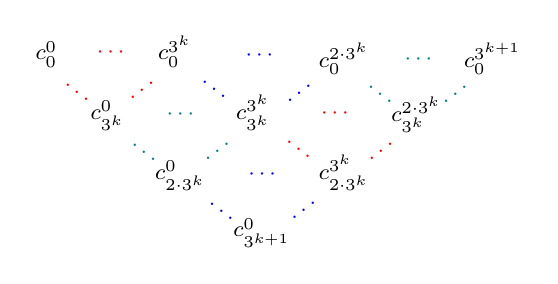
\begin{tikzpicture}
  {\footnotesize{
      % 3^(k+1)段目
      \node (a0) {$c^{0}_{3^{k+1}}$};
      % 2*3^k段目
      \node[above left=0.2cm of a0] (b0) {$c^{0}_{2\cdot3^{k}}$};
      \node[above right=0.2cm of a0] (b1) {$c^{3^{k}}_{2\cdot3^{k}}$};
      % 3^k段目
      \node[above left=0.25cm of b0] (c0) {$c^{0}_{3^{k}}$};
      \node[above right=0.25cm of b0] (c1) {$c^{3^{k}}_{3^{k}}$};
      \node[above right=0.1cm of b1] (c2) {$c^{2\cdot3^{k}}_{3^{k}}$};
      % 0段目
      \node[above left=0.3cm of c0] (d0) {$c^{0}_{0}$};
      \node[above right=0.3cm of c0] (d1) {$c^{3^{k}}_{0}$};
      \node[above left=0.1cm of c2] (d2) {$c^{2\cdot3^{k}}_{0}$};
      \node[above right=0.1cm of c2] (d3) {$c^{3^{k+1}}_{0}$};
      % 点線 [3^(k+1)段 〜 2*3^k 段]
      \node[blue] at ($(a0)!.5!(b0)$) {$\ddots$};
      \node[blue] at ($(b0)!.5!(b1)$) {$\cdots$};
      \node[blue] at ($(a0)!.5!(b1)$) {$\iddots$};
      % 点線 [2*3^k 段 〜 3^k 段]
      \node[teal] at ($(b0)!.5!(c0)$) {$\ddots$};
      \node[teal] at ($(c0)!.5!(c1)$) {$\cdots$};
      \node[teal] at ($(b0)!.5!(c1)$) {$\iddots$};
      \node[red] at ($(b1)!.5!(c1)$) {$\ddots$};
      \node[red] at ($(c1)!.5!(c2)$) {$\cdots$};
      \node[red] at ($(b1)!.5!(c2)$) {$\iddots$};
      % 点線 [3^k 段 〜 0 段]
      \node[red] at ($(c0)!.5!(d0)$) {$\ddots$};
      \node[red] at ($(d0)!.5!(d1)$) {$\cdots$};
      \node[red] at ($(c0)!.5!(d1)$) {$\iddots$};
      \node[blue] at ($(c1)!.5!(d1)$) {$\ddots$};
      \node[blue] at ($(d1)!.5!(d2)$) {$\cdots$};
      \node[blue] at ($(c1)!.5!(d2)$) {$\iddots$};
      \node[teal] at ($(c2)!.5!(d2)$) {$\ddots$};
      \node[teal] at ($(d2)!.5!(d3)$) {$\cdots$};
      \node[teal] at ($(c2)!.5!(d3)$) {$\iddots$};
  }}
\end{tikzpicture}

    \end{center}
    $k$に関する数学的帰納法を用いて証明する.
    \begin{enumerate}
    \item
      帰納法の仮定より$3^k$段の三色三角形は調和彩色三角形.
    \item
      最上段の$4$色$c^0_0, c^{3^{k}}_0, c^{2\cdot3^{k}}_0, c^{3^{k+1}}_0$ と $mix$ を用いて最下段の色が得られる.
    \item
      $mix$ の性質より,最上段の$2$色 $c^0_0, c^{3^{k+1}}_0$ を用いて最下段の色が得られる.
    \item
      $3^{k+1}$段も調和彩色三角形であることが示せた.
    \end{enumerate}
  } 
\end{frame}

\section{必要条件の証明}

\begin{frame}[fragile]
  \frametitle{必要条件の証明}
  \begin{block}{必要条件( $n$ が偶数のとき )}
    \color{red}
    {\tt{\verb|~|odd n}}
    \color{black}
    {\tt{$\Rightarrow$ \verb|~|WellColoredTriangle x n}}
  \end{block}
  {\small
    \vfill
    \begin{center}
      \begin{tabular}{c}
        % 9steps
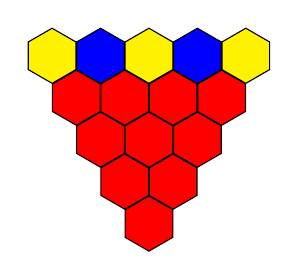
\begin{tikzpicture}[scale=0.35]
  %9段目
  \filldraw[fill=red] (0,0)--++(30:1)--++(90:1)--++(150:1)--++(210:1)--++(270:1)--cycle;
  %8段目
  \filldraw[fill=red,xshift={-25},yshift={25*sqrt(3)}] (0,0)--++(30:1)--++(90:1)--++(150:1)--++(210:1)--++(270:1)--cycle;
  \filldraw[fill=red,xshift={25},yshift={25*sqrt(3)}] (0,0)--++(30:1)--++(90:1)--++(150:1)--++(210:1)--++(270:1)--cycle;
  %7段目
  \filldraw[fill=red,xshift={-25*2},yshift={25*sqrt(3)*2}] (0,0)--++(30:1)--++(90:1)--++(150:1)--++(210:1)--++(270:1)--cycle;
  \filldraw[fill=red,yshift={25*sqrt(3)*2}] (0,0)--++(30:1)--++(90:1)--++(150:1)--++(210:1)--++(270:1)--cycle;
  \filldraw[fill=red,xshift={25*2},yshift={25*sqrt(3)*2}] (0,0)--++(30:1)--++(90:1)--++(150:1)--++(210:1)--++(270:1)--cycle;
  %6段目
  \filldraw[fill=red,xshift={-25*3},yshift={25*sqrt(3)*3}] (0,0)--++(30:1)--++(90:1)--++(150:1)--++(210:1)--++(270:1)--cycle;
  \filldraw[fill=red,xshift={-25},yshift={25*sqrt(3)*3}] (0,0)--++(30:1)--++(90:1)--++(150:1)--++(210:1)--++(270:1)--cycle;
  \filldraw[fill=red,xshift={25},yshift={25*sqrt(3)*3}] (0,0)--++(30:1)--++(90:1)--++(150:1)--++(210:1)--++(270:1)--cycle;
  \filldraw[fill=red,xshift={25*3},yshift={25*sqrt(3)*3}] (0,0)--++(30:1)--++(90:1)--++(150:1)--++(210:1)--++(270:1)--cycle;
  %5段目
  \filldraw[fill=yellow,xshift={-25*4},yshift={25*sqrt(3)*4}] (0,0)--++(30:1)--++(90:1)--++(150:1)--++(210:1)--++(270:1)--cycle;
  \filldraw[fill=blue,xshift={-25*2},yshift={25*sqrt(3)*4}] (0,0)--++(30:1)--++(90:1)--++(150:1)--++(210:1)--++(270:1)--cycle;
  \filldraw[fill=yellow,yshift={25*sqrt(3)*4}] (0,0)--++(30:1)--++(90:1)--++(150:1)--++(210:1)--++(270:1)--cycle;
  \filldraw[fill=blue,xshift={25*2},yshift={25*sqrt(3)*4}] (0,0)--++(30:1)--++(90:1)--++(150:1)--++(210:1)--++(270:1)--cycle;
  \filldraw[fill=yellow,xshift={25*4},yshift={25*sqrt(3)*4}] (0,0)--++(30:1)--++(90:1)--++(150:1)--++(210:1)--++(270:1)--cycle;
\end{tikzpicture}

        \\
        $n=4$のとき
      \end{tabular}
    \end{center}
    \begin{enumerate}
    \item
      最上段の両端のマスからそれぞれ黄,青の順で対称的に交互に塗る.
    \item
      $1$段下において,マスはすべて赤で塗られる.
    \item
      最下段のマスは赤が塗られているので矛盾.
    \end{enumerate}
  } 
\end{frame}

\begin{frame}[fragile]
  \frametitle{必要条件の証明}
  \begin{block}{必要条件( $n$ が奇数 かつ $3^k < n \leq 3^k \cdot 2$ のとき)}
    \color{red}
    {\tt{3\verb|^|k < n $\leq$ (3\verb|^|k).*2 $\Rightarrow$ odd n}}
    \color{black}
    {\tt{$\Rightarrow$ \verb|~|WellColoredTriangle x n}} 
  \end{block}
  {\footnotesize
    \vfill
    \begin{center}
      \begin{tabular}{ccc}
        \input{shortodd_steps2}
        &
        \hfill
        &
        \input{shortodd_steps3}
        \\
        $n=5$ $(k=1)$ のとき
        &
        \hfill
        &
        $n=11$ $(k=2)$ のとき
      \end{tabular}
    \end{center}
    \begin{enumerate}
    \item
      最上段の両端のマスからそれぞれ黄,青の順で対称的に交互に塗る.
    \item
      $3^k$段下において,外側から黄,青の順で対称的に交互に塗られる.
    \item
      さらに,$1$段(最上段から$3^k + 1$段)下において,マスはすべて赤で塗られる.
    \item
      最下段のマスは赤が塗られているので矛盾.
    \end{enumerate}
  } 
\end{frame}

\begin{frame}[fragile]
  \frametitle{必要条件の証明}
  \begin{block}{必要条件( $n$ が奇数 かつ $3^k \cdot 2 + 1 \leq n < 3^{k+1}$ のとき)}
    \color{red}
    {\tt{(3\verb|^|k).*2.+1 $\leq$ n < 3\verb|^|k.+1}}
    \color{black}      
    {\tt{$\Rightarrow$ \verb|~|WellColoredTriangle x n}}
  \end{block}
  {\footnotesize
    \vfill
    \begin{center}
      \begin{tabular}{c}
        % 9steps
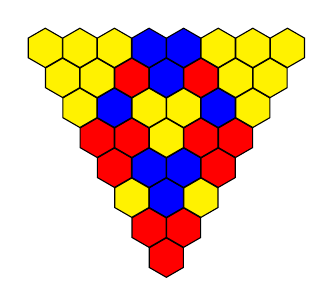
\begin{tikzpicture}[scale=0.25]
  %9段目
  \filldraw[fill=red] (0,0)--++(30:1)--++(90:1)--++(150:1)--++(210:1)--++(270:1)--cycle;
  %8段目
  \filldraw[fill=red,xshift={-25},yshift={25*sqrt(3)}] (0,0)--++(30:1)--++(90:1)--++(150:1)--++(210:1)--++(270:1)--cycle;
  \filldraw[fill=red,xshift={25},yshift={25*sqrt(3)}] (0,0)--++(30:1)--++(90:1)--++(150:1)--++(210:1)--++(270:1)--cycle;
  %7段目
  \filldraw[fill=yellow,xshift={-25*2},yshift={25*sqrt(3)*2}] (0,0)--++(30:1)--++(90:1)--++(150:1)--++(210:1)--++(270:1)--cycle;
  \filldraw[fill=blue,yshift={25*sqrt(3)*2}] (0,0)--++(30:1)--++(90:1)--++(150:1)--++(210:1)--++(270:1)--cycle;
  \filldraw[fill=yellow,xshift={25*2},yshift={25*sqrt(3)*2}] (0,0)--++(30:1)--++(90:1)--++(150:1)--++(210:1)--++(270:1)--cycle;
  %6段目
  \filldraw[fill=red,xshift={-25*3},yshift={25*sqrt(3)*3}] (0,0)--++(30:1)--++(90:1)--++(150:1)--++(210:1)--++(270:1)--cycle;
  \filldraw[fill=blue,xshift={-25},yshift={25*sqrt(3)*3}] (0,0)--++(30:1)--++(90:1)--++(150:1)--++(210:1)--++(270:1)--cycle;
  \filldraw[fill=blue,xshift={25},yshift={25*sqrt(3)*3}] (0,0)--++(30:1)--++(90:1)--++(150:1)--++(210:1)--++(270:1)--cycle;
  \filldraw[fill=red,xshift={25*3},yshift={25*sqrt(3)*3}] (0,0)--++(30:1)--++(90:1)--++(150:1)--++(210:1)--++(270:1)--cycle;
  %5段目
  \filldraw[fill=red,xshift={-25*4},yshift={25*sqrt(3)*4}] (0,0)--++(30:1)--++(90:1)--++(150:1)--++(210:1)--++(270:1)--cycle;
  \filldraw[fill=red,xshift={-25*2},yshift={25*sqrt(3)*4}] (0,0)--++(30:1)--++(90:1)--++(150:1)--++(210:1)--++(270:1)--cycle;
  \filldraw[fill=yellow,yshift={25*sqrt(3)*4}] (0,0)--++(30:1)--++(90:1)--++(150:1)--++(210:1)--++(270:1)--cycle;
  \filldraw[fill=red,xshift={25*2},yshift={25*sqrt(3)*4}] (0,0)--++(30:1)--++(90:1)--++(150:1)--++(210:1)--++(270:1)--cycle;
  \filldraw[fill=red,xshift={25*4},yshift={25*sqrt(3)*4}] (0,0)--++(30:1)--++(90:1)--++(150:1)--++(210:1)--++(270:1)--cycle;
  %4段目
  \filldraw[fill=yellow,xshift={-25*5},yshift={25*sqrt(3)*5}] (0,0)--++(30:1)--++(90:1)--++(150:1)--++(210:1)--++(270:1)--cycle;
  \filldraw[fill=blue,xshift={-25*3},yshift={25*sqrt(3)*5}] (0,0)--++(30:1)--++(90:1)--++(150:1)--++(210:1)--++(270:1)--cycle;
  \filldraw[fill=yellow,xshift={-25*1},yshift={25*sqrt(3)*5}] (0,0)--++(30:1)--++(90:1)--++(150:1)--++(210:1)--++(270:1)--cycle;
  \filldraw[fill=yellow,xshift={25*1},yshift={25*sqrt(3)*5}] (0,0)--++(30:1)--++(90:1)--++(150:1)--++(210:1)--++(270:1)--cycle;
  \filldraw[fill=blue,xshift={25*3},yshift={25*sqrt(3)*5}] (0,0)--++(30:1)--++(90:1)--++(150:1)--++(210:1)--++(270:1)--cycle;
  \filldraw[fill=yellow,xshift={25*5},yshift={25*sqrt(3)*5}] (0,0)--++(30:1)--++(90:1)--++(150:1)--++(210:1)--++(270:1)--cycle;
  %3段目
  \filldraw[fill=yellow,xshift={-25*6},yshift={25*sqrt(3)*6}] (0,0)--++(30:1)--++(90:1)--++(150:1)--++(210:1)--++(270:1)--cycle;
  \filldraw[fill=yellow,xshift={-25*4},yshift={25*sqrt(3)*6}] (0,0)--++(30:1)--++(90:1)--++(150:1)--++(210:1)--++(270:1)--cycle;
  \filldraw[fill=red,xshift={-25*2},yshift={25*sqrt(3)*6}] (0,0)--++(30:1)--++(90:1)--++(150:1)--++(210:1)--++(270:1)--cycle;
  \filldraw[fill=blue,yshift={25*sqrt(3)*6}] (0,0)--++(30:1)--++(90:1)--++(150:1)--++(210:1)--++(270:1)--cycle;
  \filldraw[fill=red,xshift={25*2},yshift={25*sqrt(3)*6}] (0,0)--++(30:1)--++(90:1)--++(150:1)--++(210:1)--++(270:1)--cycle;
  \filldraw[fill=yellow,xshift={25*4},yshift={25*sqrt(3)*6}] (0,0)--++(30:1)--++(90:1)--++(150:1)--++(210:1)--++(270:1)--cycle;
  \filldraw[fill=yellow,xshift={25*6},yshift={25*sqrt(3)*6}] (0,0)--++(30:1)--++(90:1)--++(150:1)--++(210:1)--++(270:1)--cycle;
  %2段目
  \filldraw[fill=yellow,xshift={-25*7},yshift={25*sqrt(3)*7}] (0,0)--++(30:1)--++(90:1)--++(150:1)--++(210:1)--++(270:1)--cycle;
  \filldraw[fill=yellow,xshift={-25*5},yshift={25*sqrt(3)*7}] (0,0)--++(30:1)--++(90:1)--++(150:1)--++(210:1)--++(270:1)--cycle;
  \filldraw[fill=yellow,xshift={-25*3},yshift={25*sqrt(3)*7}] (0,0)--++(30:1)--++(90:1)--++(150:1)--++(210:1)--++(270:1)--cycle;
  \filldraw[fill=blue,xshift={-25*1},yshift={25*sqrt(3)*7}] (0,0)--++(30:1)--++(90:1)--++(150:1)--++(210:1)--++(270:1)--cycle;
  \filldraw[fill=blue,xshift={25*1},yshift={25*sqrt(3)*7}] (0,0)--++(30:1)--++(90:1)--++(150:1)--++(210:1)--++(270:1)--cycle;
  \filldraw[fill=yellow,xshift={25*3},yshift={25*sqrt(3)*7}] (0,0)--++(30:1)--++(90:1)--++(150:1)--++(210:1)--++(270:1)--cycle;
  \filldraw[fill=yellow,xshift={25*5},yshift={25*sqrt(3)*7}] (0,0)--++(30:1)--++(90:1)--++(150:1)--++(210:1)--++(270:1)--cycle;
  \filldraw[fill=yellow,xshift={25*7},yshift={25*sqrt(3)*7}] (0,0)--++(30:1)--++(90:1)--++(150:1)--++(210:1)--++(270:1)--cycle;
\end{tikzpicture}

        \\
        $n=7$ $(k=1)$ のとき
      \end{tabular}
    \end{center}
    \begin{enumerate}
    \item
      最上段の両端のマスからそれぞれ$3^k$マス内を黄,その他を青で対称的に塗る.
    \item
      $3^k$段下において,外側から$ n - 2 \cdot 3^k + 1$ マスはすべて赤で塗られる.
    \item
      さらに,$3^k$段(最上段から$2 \cdot 3^k$段)下において,マスはすべて赤で塗られる.
    \item
      最下段のマスは赤が塗られているので矛盾.
    \end{enumerate}
  } 
\end{frame}

\section{まとめ}

\begin{frame}[fragile]
  \frametitle{研究のまとめ}
  \begin{block}{研究の成果}
    {\tt{n > 0 $\Rightarrow$ ($\exists$k, n = 3\verb|^|k) $\Leftrightarrow$ WellColoredTriangle x n}}
    を Coq で証明した.
  \end{block}
  \vfill
  \begin{alertblock}{問題であった点}
    \begin{itemize}
    \item
      幾何的な問題をどのようにして形式化するか
    \item
      暗黙のうちに仮定されてしまっていることを見落としやすい
    \end{itemize}
  \end{alertblock}
  \vfill
  \textbf{[解決法・工夫点]}
  \begin{itemize}
  \item
    三角形三色問題の暗黙の前提を明確化
  \item
    幾何的な状況を関数を用いて論理式で表現
  \end{itemize}
\end{frame}

\begin{frame}
  \frametitle{中間発表のまとめ}
  \begin{exampleblock}{2021年4月現在}
    \begin{itemize}
    \item 卒業論文(学部)
    \item 三角形三色問題の十分条件のみを形式化
    \item コード数は約380行  
    \end{itemize}
  \end{exampleblock}
  \vfill
  \begin{block}{2021年2月現在}
    \begin{itemize}
    \item
      日本ソフトウェア科学会第38回にて発表
    \item
      『Coqによる三角形三色問題』として論文を投稿中
    \item
      Coq を用いて三角形三色問題の必要十分条件を形式化
    \item
      Coq の拡張ライブラリ(SSReflect)を用いてコードを改良
    \item
      コード数は約360行
    \end{itemize}
  \end{block}
  \vfill
\end{frame}

% 参考文献
\begin{frame}
  \frametitle{参考文献}
  \begin{thebibliography}{99}
  \bibitem{Coq}
    ``The Coq Proof Assistant'',
    https://coq.inria.fr/. 

  \bibitem{SSReflect}
    ``The SSReflect proof language'',
    \\
    https://coq.inria.fr/refman/proof-engine/ssreflect-proof-language.html. 
    
  \bibitem{CoqBook}
    萩原学, アフェルド・レナルド, 
    ``Coq/SSReflect/MathComp による定理証明'',
    森北出版,
    2018. 
    
  \bibitem{Nishiyama1}
    西山豊,
    ``エレガントな解答をもとむ 出題2'',
    数学セミナー,
    4月号, pp.87--91, 2013.
    
  \bibitem{Nishiyama2}
    西山豊,
    ``数学を楽しむ/三角形三色問題'',
    現代数学,
    Vol.47, No.10, pp.36--41, 2014.
    
  \bibitem{Nishiyama3}
    Y.~Nishiyama,
    ``THE THREE-COLOR TRIANGLE PROBLEM'', 
    International Journal of Pure and Applied Mathematics,
    Vol.85, No.1, pp.69--81, 2013.
  \end{thebibliography}
\end{frame}

\end{document}

%memo
%1ページずつ伝えることを決める.→事前に紙に設計図を書いておく.
%スライドの1枚目は背景や目的を書く.
%(専門用語は簡単な説明をのせておけばよい→詳しい話はスライドの後半に載せる)
%この次のページは研究成果やできると何が良いのかを書く.

%公理化したのは工夫ポイント.(重要)

%定義,公理や証明は論文の切り貼りでも大丈夫→ただし,スライドの冒頭の説明がより伝わるようにすること.
